%%%%%%%%%%%%%%%%%%%%%%%%%%%%%%%%%%%%%%%%%%%%%%%%%%%%%%%%%%%%%%%%%%%%%%%%%%%%%%%%
%%%%%%%%%%%%%%%%%%%%%%%%%%%%%%%%%%%%%%%%%%%%%%%%%%%%%%%%%%%%%%%%%%%%%%%%%%%%%%%%
%%% Template for AIMS Rwanda Assignments         %%%              %%%
%%% Author:   AIMS Rwanda tutors                             %%%   ###        %%%
%%% Email: tutors2017-18@aims.ac.rw                               %%%   ###        %%%
%%% Copyright: This template was designed to be used for    %%% #######      %%%
%%% the assignments at AIMS Rwanda during the academic year %%%   ###        %%%
%%% 2017-2018.                                              %%%   #########  %%%
%%% You are free to alter any part of this document for     %%%   ###   ###  %%%
%%% yourself and for distribution.                          %%%   ###   ###  %%%
%%%                                                         %%%              %%%
%%%%%%%%%%%%%%%%%%%%%%%%%%%%%%%%%%%%%%%%%%%%%%%%%%%%%%%%%%%%%%%%%%%%%%%%%%%%%%%%
%%%%%%%%%%%%%%%%%%%%%%%%%%%%%%%%%%%%%%%%%%%%%%%%%%%%%%%%%%%%%%%%%%%%%%%%%%%%%%%%


%%%%%% Ensure that you do not write the questions before each of the solutions because it is not necessary. %%%%%% 

\documentclass[12pt,a4paper]{article}

%%%%%%%%%%%%%%%%%%%%%%%%% packages %%%%%%%%%%%%%%%%%%%%%%%%
\usepackage{amsmath}
\usepackage{amssymb}
\usepackage{amsthm}
\usepackage{amsfonts}
\usepackage{graphicx}
\usepackage[all]{xy}
\usepackage{tikz}
\usepackage{verbatim}
\usepackage{float}
\usepackage[left=2cm,right=2cm,top=3cm,bottom=2.5cm]{geometry}
\usepackage{hyperref}
\usepackage{caption}
\usepackage{subcaption}
\usepackage{psfrag}
\usepackage{mathrsfs}
\usepackage{actuarialangle}
\usepackage[T1]{fontenc}
\usepackage{float}
%%%%%%%%%%%%%%%%%%%%% students data %%%%%%%%%%%%%%%%%%%%%%%%
\newcommand{\student}{Yusuf Brima}
\newcommand{\course}{Fluid Mechanics}
\newcommand{\assignment}{2}

%%%%%%%%%%%%%%%%%%% using theorem style %%%%%%%%%%%%%%%%%%%%
\newtheorem{thm}{Theorem}
\newtheorem{lem}[thm]{Lemma}
\newtheorem{defn}[thm]{Definition}
\newtheorem{exa}[thm]{Example}
\newtheorem{rem}[thm]{Remark}
\newtheorem{coro}[thm]{Corollary}
\newtheorem{quest}{Question}[section]

%%%%%%%%%%%%%%  Shortcut for usual set of numbers  %%%%%%%%%%%

\newcommand{\N}{\mathbb{N}}
\newcommand{\Z}{\mathbb{Z}}
\newcommand{\Q}{\mathbb{Q}}
\newcommand{\R}{\mathbb{R}}
\newcommand{\C}{\mathbb{C}}

%%%%%%%%%%%%%%%%%%%%%%%%%%%%%%%%%%%%%%%%%%%%%%%%%%%%%%%555
\begin{document}

%%%%%%%%%%%%%%%%%%%%%%% title page %%%%%%%%%%%%%%%%%%%%%%%%%%
\thispagestyle{empty}
%\begin{figure}
%    \centering
%    \includegraphics[width=\textwidth]{aims_rwanda.jpg}
%\end{figure}
\begin{center}
\textbf{AFRICAN INSTITUTE FOR MATHEMATICAL SCIENCES \\[0.5cm]
(AIMS RWANDA, KIGALI)}
\vspace{1.0cm}
\end{center}

%%%%%%%%%%%%%%%%%%%%% assignment information %%%%%%%%%%%%%%%%
\noindent
\rule{17cm}{0.2cm}\\[0.3cm]
Name: \student \hfill Assignment Number: \assignment\\[0.1cm]
Course: \course \hfill Date: \today\\
\rule{17cm}{0.05cm}
\vspace{1.0cm}
\section*{Exercise 1}

\begin{enumerate}
		\item[(i)] Given the dynamical systems in \eqref{eq:1}, the $4^{th}$ order Runge-Kutta solution is plotted below.
				\begin{equation}
						  \frac{d\mathbf{x}}{dt} =  \begin{pmatrix}
		  								5 &  1\\
		  								3 & 1
		  						\end{pmatrix} \mathbf{x}
						\label{eq:1}
			  \end{equation}
					\begin{figure}[!h]
									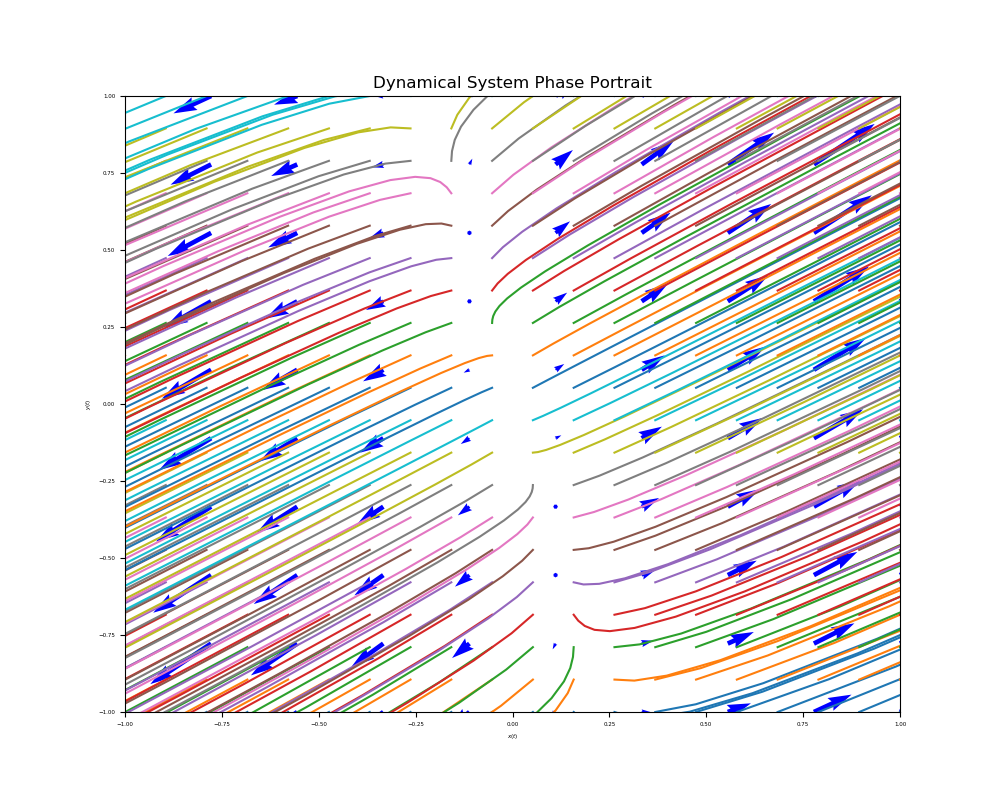
\includegraphics[width=430pt,  height=230pt]{./graphics/q001_a.png}
										\caption{A plot of the dynamical system of ODEs using RK4 method}
										\label{fig:q1}
								\end{figure}
					\item[(ii)] Given the dynamical systems in \eqref{eq:2}, the $4^{th}$ order Runge-Kutta solution is plotted below.
				\begin{equation}
						  \frac{d\mathbf{x}}{dt} =  \begin{pmatrix}
		  								2 &  -5\\
		  								1  & -2
		  						\end{pmatrix} \mathbf{x}
						\label{eq:2}
			  \end{equation}
					\begin{figure}[!h]
									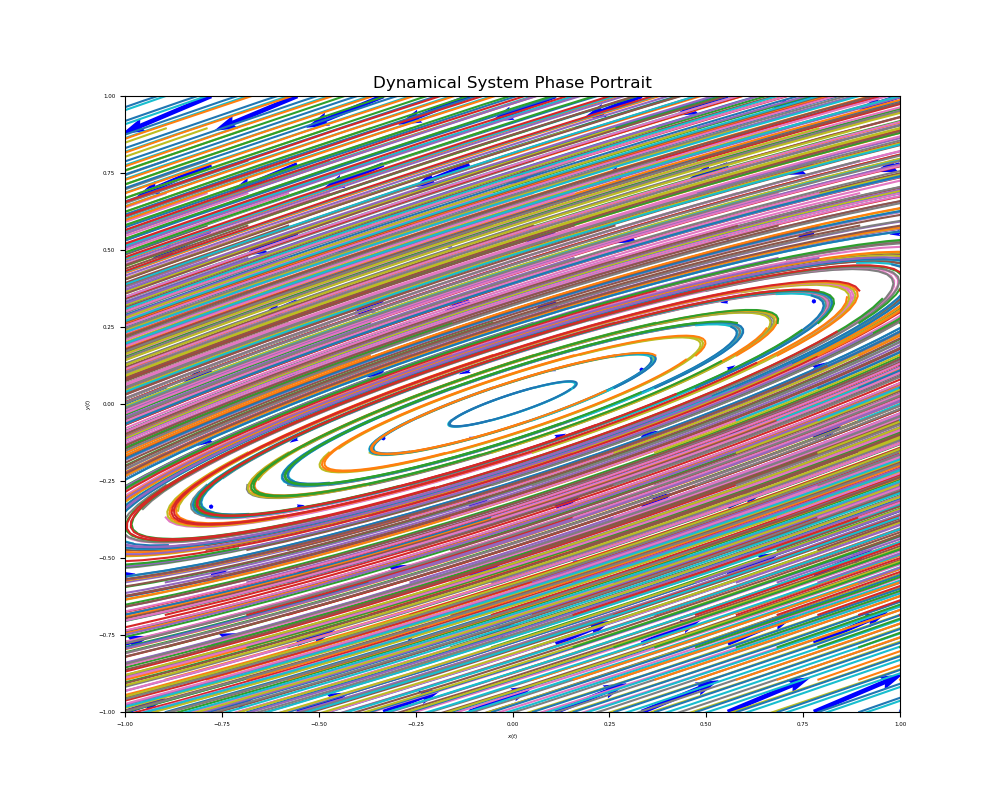
\includegraphics[width=430pt,  height=200pt]{./graphics/q001_b.png}
										\caption{A plot of the dynamical system of ODEs using RK4 method}
										\label{fig:q2}
								\end{figure}
					\item[(iii)] Given the dynamical systems in \eqref{eq:3}, the $4^{th}$ order Runge-Kutta solution is plotted below.
				\begin{equation}
						  \frac{d\mathbf{x}}{dt} =  \begin{pmatrix}
		  								1 &  -5\\
		  								1 & -3
		  						\end{pmatrix} \mathbf{x}
						\label{eq:3}
			  \end{equation}
					\begin{figure}[!h]
									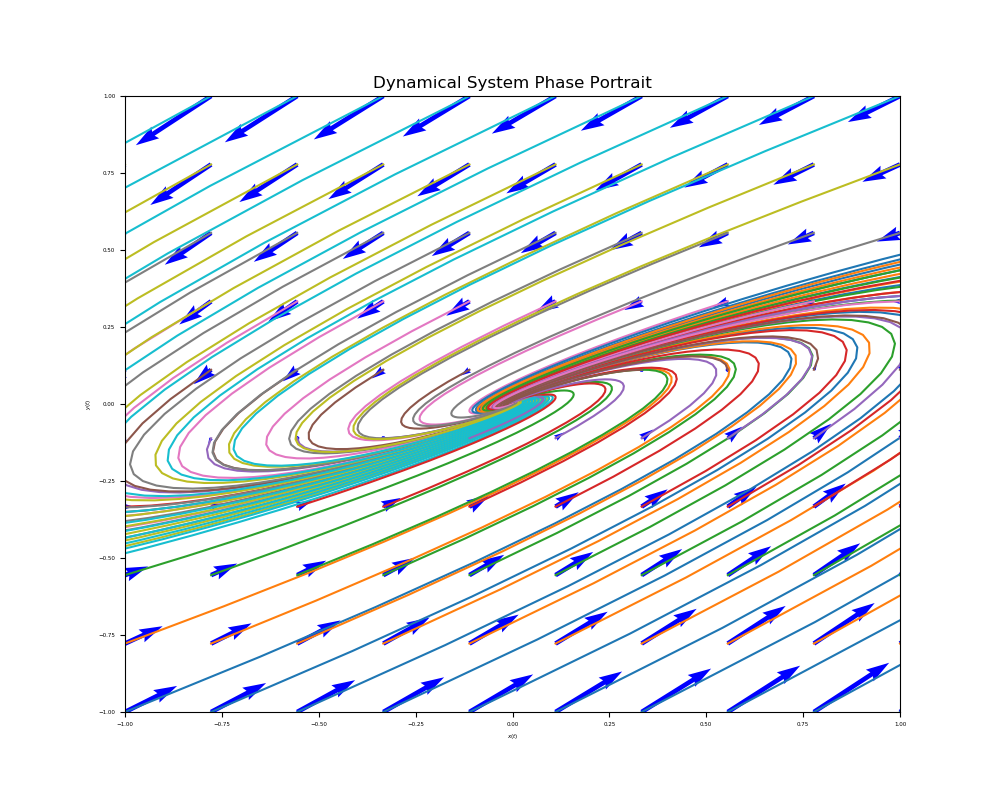
\includegraphics[width=430pt,  height=200pt]{./graphics/q001_c.png}
										\caption{A plot of the dynamical system of ODEs using RK4 method}
										\label{fig:q3}
								\end{figure}
								\item[(iv)] Given the dynamical systems in \eqref{eq:4}, the $4^{th}$ order Runge-Kutta solution is plotted below.
				\begin{equation}
						  \frac{d\mathbf{x}}{dt} =  \begin{pmatrix}
		  								2 &  -1\\
		  								 3 &  -2
		  						\end{pmatrix} \mathbf{x}
						\label{eq:4}
			  \end{equation}
					\begin{figure}[!h]
									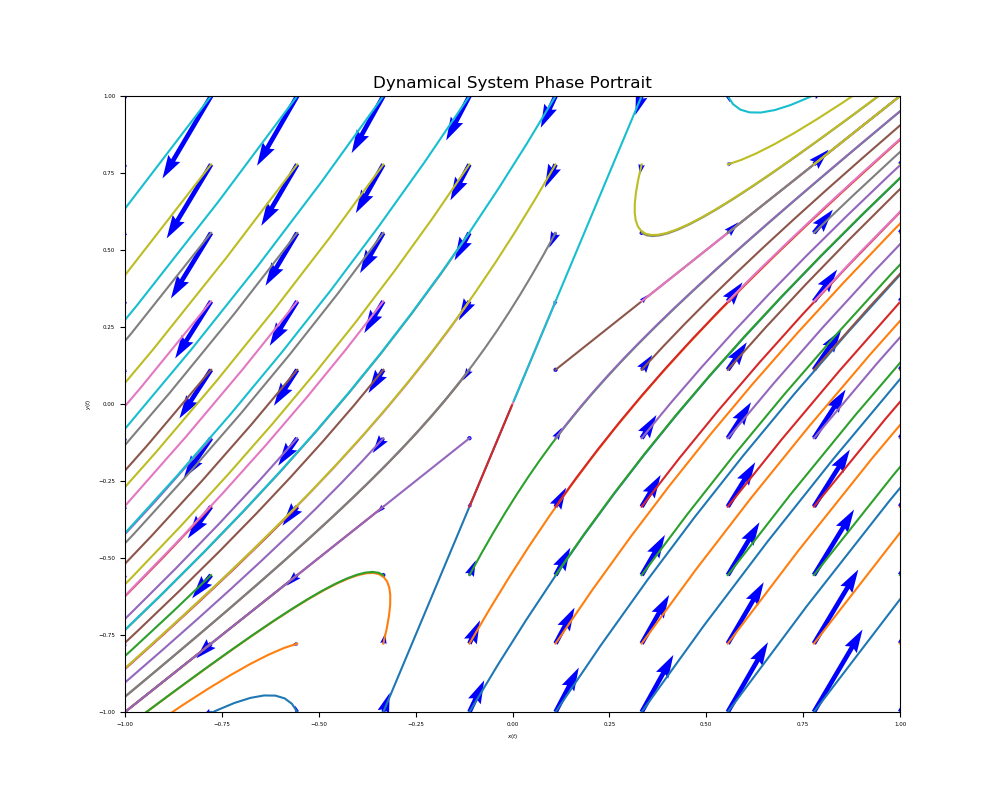
\includegraphics[width=430pt,  height=200pt]{./graphics/q001_d.png}
										\caption{A plot of the dynamical system of ODEs using RK4 method}
										\label{fig:q4}
								\end{figure}
\end{enumerate}
\section*{Exercise 2}
Given 
\begin{equation}
		\frac{dx}{dt} =  y - x^2, \quad
		\frac{dy}{dt} = x -2
		\label{eq:5}
\end{equation}
\begin{enumerate}
							\item[(i)]   We calculate the equilibrium point as thus:
							\item[(ii)]We proceed as follows to linearize the dynamical system around the equilibrium in \eqref{eq:5}.
							\item[(iii)] We find the eigenvalue and eigenvector of the linearized system,  and the character of the equilibrium.
							\item[(iv)] Given the dynamical systems above the $4^{th}$ order Runge-Kutta solution is plotted below.

					\begin{figure}[!h]
									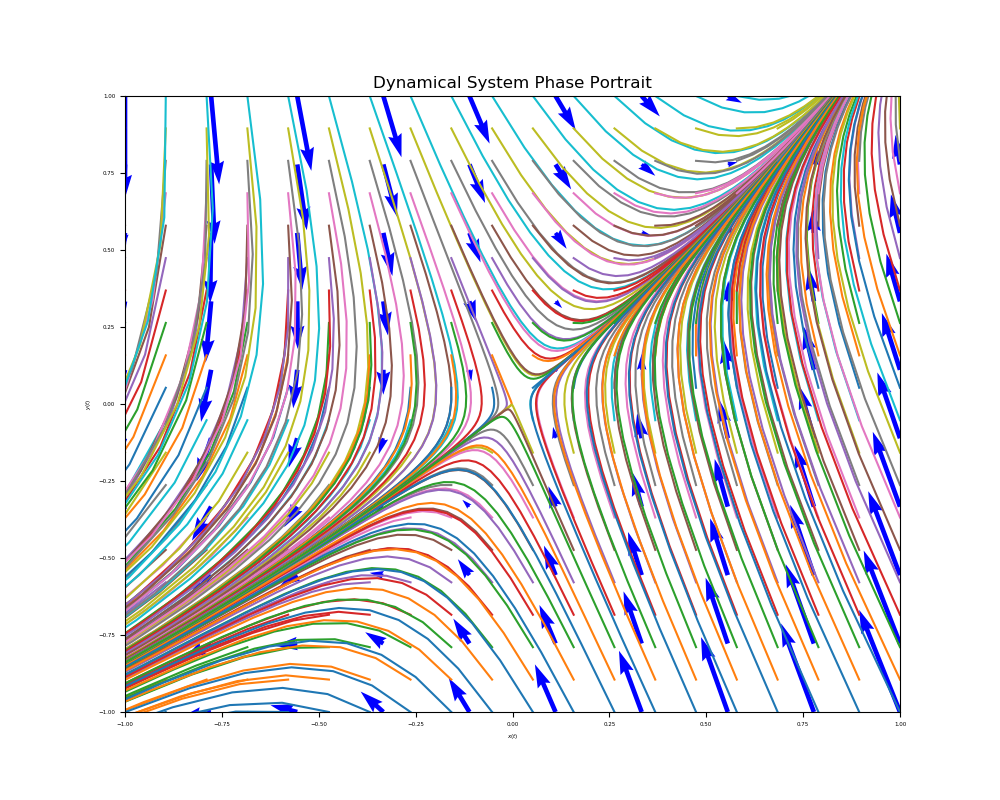
\includegraphics[width=430pt,  height=200pt]{./graphics/q002_a.png}
										\caption{A plot of the dynamical system of ODEs using RK4 method}
										\label{fig:q5}
								\end{figure}
\end{enumerate}
\end{document}